\appendix

\section{Locality-boosting analysis}

I'll take care of this section. Maciek.


Definitions are in Section~\ref{sec:locality-boosting}

Locality-boosting gains depend on the ability to choose a partitioning that isolates requests with similar access patterns.
Consider a self-adjusting list
storing a set of items $\{ 1, 2, 3, 4, 5, 6 \}$, and consider a request sequence $\sigma = \langle 1, 2, 3, 1, 2, 3, 1, 2, 3, \ldots \rangle$.
If the items are stored in a single self-adjusting list with a Move-To-Front reorganization operation, the three requested items $\{1,2,3\}$ compete for the front of the list, and incur the cost of three comparisons per each request.
However, if we partition the items into three lists with a partitioning function that assigns the items $\{1, 2, 3\}$ to different lists, then the requested items would occupy the front of their respective lists, resulting in one comparison per request.

\subsection{Analysis}
% \subsubsection{Absolute costs for a single self-adjusting list.}
% Self-adjusting lists are often analyzed within the framework \emph{competitive analysis}~\cite{Borodin98}, where we compare the online algorithm's performance to an offline optimum for the sequence.
% However, in this work we are interested in absolute costs.

Albers and Lauer~\cite{AlbersL16} characterized the absolute cost of serving a request sequence $\sigma$ in terms of the number of \emph{runs} in $\sigma$.
Runs are defined for two-item input sequences, and to characterize sequences consisting of more items, we sum the number of runs in sequences with all but two items removed, for all pairs of items.

\begin{definition}
	Let L be the set of items in the list to be maintained. Consider a fixed request sequence~$\sigma$. For any two items $x, y \in L$
	with $x \neq y$, let $\sigma_{xy}$ be the request sequence that is derived from $\sigma$ by deleting all requests that are neither to x nor
	to y.
\end{definition}

\begin{definition}
	Any maximal subsequence of consecutive requests to the same item in $\sigma_{xy}$ is called a run. Let $r(\sigma_{xy})$ be the number of runs in $\sigma_{xy}$. 
	We define $r(\sigma) = \sum_{x,y : x \neq y} r(\sigma_{xy})$.
\end{definition}
%
Then, the cost of Move-To-Front can be upper-bounded in terms of number of runs:
%
\begin{theorem}
	For any sequence $\sigma$ the cost incurred on a single list by MTF is 
	$MTF(\sigma) \le r(\sigma) + |\sigma|$.
	\label{thm:mtf-runs}
\end{theorem}
The proof of the above theorem is due to Albers and Lauer~\cite{AlbersL16}.

The above characterization in terms of runs can be extended to partitioned self-adjusting lists running Move-To-Front.
\begin{lemma}
	For each list $L_i$, let $\sigma^{(h(\cdot) = i)}$ be a subsequence of the input $\sigma$ that contains only requests to the items assigned by $h$ to $L_i$.
	The total absolute cost incurred is then:
	$$
	MTF_h(\sigma) \le (\sum_{1 \le i \le m} r(\sigma^{(h(\cdot) = i)})) + |\sigma|
	$$
	\label{lem:parallel-cost-mtf}
\end{lemma}
\begin{proof}
	The proof follows by summing up the cost of Move-To-Front in each individual list, followed by Theorem~\ref{thm:mtf-runs}:
	
	$$ MTF_h(\sigma) \le \sum_{1 \le i \le k} (r(\sigma^{(h(\cdot) = i)}) + |\sigma^{(h(\cdot) = i)}|) = (\sum_{1 \le i \le k} r(\sigma^{(h(\cdot) = i)})) + |\sigma|,$$
	where the last step follows as $h$ is a function, and it assigns each item to only one list.
\end{proof}
The above cost characterization depends then on $h$, the assignment of items to lists.

We compare the cost incurred by the parallel lists $MTF_h(\sigma)$ to the cost incurred on a single list, $MTF(\sigma)$, in terms of the function $h$.
To this end, we define a \emph{run graph} of a sequence $\sigma$.
\begin{definition}
	For a given sequence $\sigma$, a \emph{run graph} is a complete weighted graph on $n$ vertices, where the weight of an edge $(x,y)$ is $r(\sigma_{xy})$.
\end{definition}

For an example of a run graph with hash functions, see Figure~\ref{fig:example}.
In this example, we consider two partitioned lists containing four items $a,b,c$ and $d$, and an input sequence $\sigma := abababacacaccacacadc$, $|\sigma| = 20$.
Then, $\sigma_{ab} = abababaaaaaa$ consist of $7$ runs, $\sigma_{ac} = aaaacacaccacacac$ consists of 12 runs, 
$\sigma_{ad} = aaaaaaaaad$ consists of 2 runs, 
$\sigma_{bc} = bbbccccccc$ consists of 2 runs,  $\sigma_{bd} = bbbd$ consist of 2 runs and $\sigma_{cd} := ccccccdc$ consists of 3 runs.
Figure~\ref{fig:example} depicts the run graph for $\sigma$ and two examples of functions $h_1$ and $h_2$, with $w(C_{h_1}) = 18$ and $w(C_{h_2}) = 21$ being the savings from choosing an assignment $h_1$ or $h_2$, respectively.


\begin{figure}[h!]
	\center
	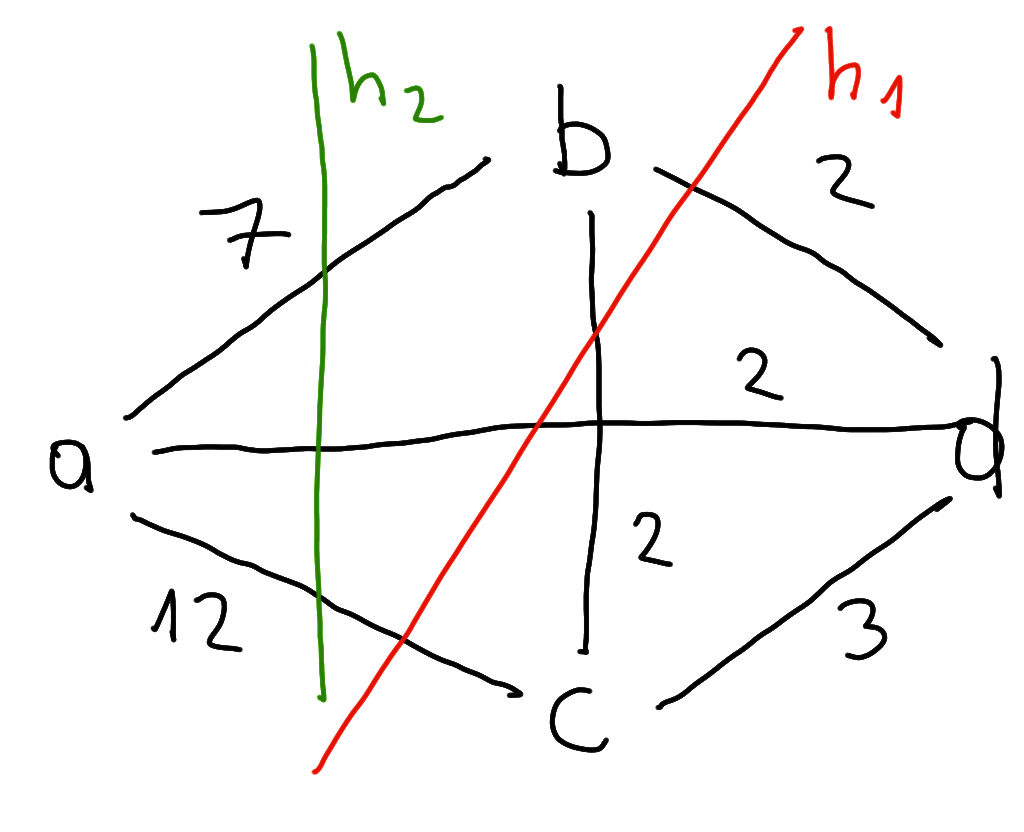
\includegraphics[width=0.5\textwidth]{./fig/cut.png}
	\caption{The run graph for $\sigma = abababacacaccacacadc$ and two examples of functions $h_1$ and $h_2$, with $w(C_{h_1}) = 18$ and $w(C_{h_2}) = 21$.}
	\label{fig:example}
\end{figure}




The run graph helps in characterizing the gains from the partitioning schema.
Each function $h$ induces a $k$-way cut of the run graph, denoted $C_h$.
With this characterization, we express the cost of parallel lists in comparison to the cost of a single list.
\begin{observation}
	Let $M$ be the cost incurred by $MTF$ operating on a single list.
	Then, the cost incurred by parallel $MTF_h$ is at most $M - w(C_h)$, where $w(C_h)$ is the total weight of the $k$-way cut $C_h$ induced by $h$.
\end{observation}

The observation follows by summing up the costs for individual lists with Lemma~\ref{lem:parallel-cost-mtf}.

Note that we ignore the cost of computing the hash function, and account only for item comparisons.


%%% Local Variables:
%%% mode: latex
%%% TeX-master: "distributed_mrf"
%%% End:
